\documentclass[14pt]{extbook}
\usepackage{multicol, enumerate, enumitem, hyperref, color, soul, setspace, parskip, fancyhdr} %General Packages
\usepackage{amssymb, amsthm, amsmath, latexsym, units, mathtools} %Math Packages
\everymath{\displaystyle} %All math in Display Style
% Packages with additional options
\usepackage[headsep=0.5cm,headheight=12pt, left=1 in,right= 1 in,top= 1 in,bottom= 1 in]{geometry}
\usepackage[usenames,dvipsnames]{xcolor}
\usepackage{dashrule}  % Package to use the command below to create lines between items
\newcommand{\litem}[1]{\item#1\hspace*{-1cm}\rule{\textwidth}{0.4pt}}
\pagestyle{fancy}
\lhead{Progress Quiz 6}
\chead{}
\rhead{Version A}
\lfoot{9689-6866}
\cfoot{}
\rfoot{Spring 2021}
\begin{document}

\begin{enumerate}
\litem{
Construct the lowest-degree polynomial given the zeros below. Then, choose the intervals that contain the coefficients of the polynomial in the form $ax^3+bx^2+cx+d$.\[ \frac{7}{3}, \frac{-5}{2}, \text{ and } \frac{-2}{3} \]\begin{enumerate}[label=\Alph*.]
\item \( a \in [16, 21], b \in [-17, -12], c \in [-104, -99], \text{ and } d \in [68, 73] \)
\item \( a \in [16, 21], b \in [11, 20], c \in [-104, -99], \text{ and } d \in [-70, -68] \)
\item \( a \in [16, 21], b \in [8, 14], c \in [-111, -104], \text{ and } d \in [-70, -68] \)
\item \( a \in [16, 21], b \in [11, 20], c \in [-104, -99], \text{ and } d \in [68, 73] \)
\item \( a \in [16, 21], b \in [96, 104], c \in [162, 167], \text{ and } d \in [68, 73] \)

\end{enumerate} }
\litem{
Describe the zero behavior of the zero $x = -2$ of the polynomial below.\[ f(x) = 2(x + 2)^{8}(x - 2)^{11}(x + 9)^{3}(x - 9)^{6} \]\begin{enumerate}[label=\Alph*.]
\begin{multicols}{2}\item 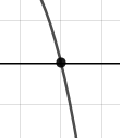
\includegraphics[width = 0.3\textwidth]{../Figures/polyZeroBehaviorAA.png}\item 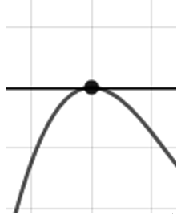
\includegraphics[width = 0.3\textwidth]{../Figures/polyZeroBehaviorBA.png}\item 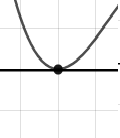
\includegraphics[width = 0.3\textwidth]{../Figures/polyZeroBehaviorCA.png}\item 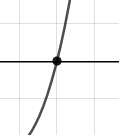
\includegraphics[width = 0.3\textwidth]{../Figures/polyZeroBehaviorDA.png}\end{multicols}\item None of the above.
\end{enumerate} }
\litem{
Which of the following equations \textit{could} be of the graph presented below?
\begin{center}
    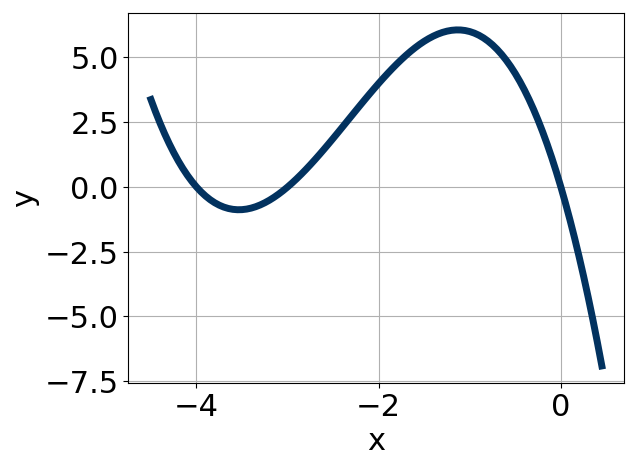
\includegraphics[width=0.5\textwidth]{../Figures/polyGraphToFunctionA.png}
\end{center}
\begin{enumerate}[label=\Alph*.]
\item \( 19x^{10} (x + 2)^{10} (x - 2)^{7} \)
\item \( -4x^{7} (x + 2)^{8} (x - 2)^{5} \)
\item \( -6x^{9} (x + 2)^{6} (x - 2)^{4} \)
\item \( 8x^{5} (x + 2)^{10} (x - 2)^{7} \)
\item \( 5x^{4} (x + 2)^{9} (x - 2)^{7} \)

\end{enumerate} }
\litem{
Describe the zero behavior of the zero $x = 7$ of the polynomial below.\[ f(x) = -2(x + 9)^{10}(x - 9)^{8}(x + 7)^{8}(x - 7)^{5} \]\begin{enumerate}[label=\Alph*.]
\begin{multicols}{2}\item 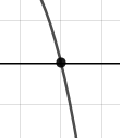
\includegraphics[width = 0.3\textwidth]{../Figures/polyZeroBehaviorCopyAA.png}\item 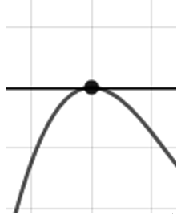
\includegraphics[width = 0.3\textwidth]{../Figures/polyZeroBehaviorCopyBA.png}\item 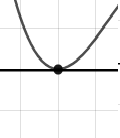
\includegraphics[width = 0.3\textwidth]{../Figures/polyZeroBehaviorCopyCA.png}\item 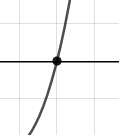
\includegraphics[width = 0.3\textwidth]{../Figures/polyZeroBehaviorCopyDA.png}\end{multicols}\item None of the above.
\end{enumerate} }
\litem{
Which of the following equations \textit{could} be of the graph presented below?
\begin{center}
    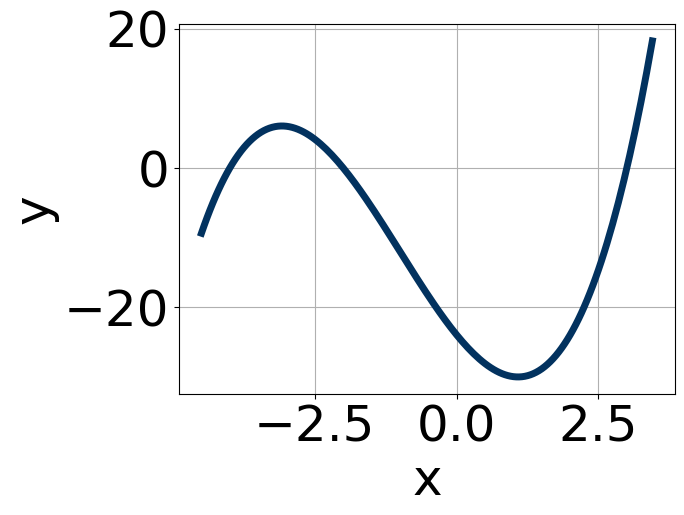
\includegraphics[width=0.5\textwidth]{../Figures/polyGraphToFunctionCopyA.png}
\end{center}
\begin{enumerate}[label=\Alph*.]
\item \( -10x^{8} (x - 3)^{5} (x + 2)^{7} \)
\item \( -5x^{8} (x - 3)^{9} (x + 2)^{4} \)
\item \( 12x^{4} (x - 3)^{11} (x + 2)^{11} \)
\item \( 11x^{4} (x - 3)^{10} (x + 2)^{7} \)
\item \( 19x^{7} (x - 3)^{8} (x + 2)^{9} \)

\end{enumerate} }
\litem{
Describe the end behavior of the polynomial below.\[ f(x) = -5(x - 9)^{3}(x + 9)^{6}(x - 7)^{3}(x + 7)^{5} \]\begin{enumerate}[label=\Alph*.]
\begin{multicols}{2}\item 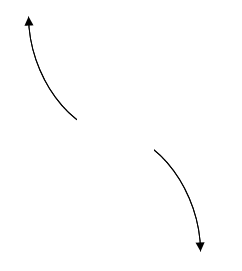
\includegraphics[width = 0.3\textwidth]{../Figures/polyEndBehaviorCopyAA.png}\item 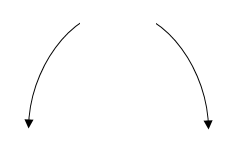
\includegraphics[width = 0.3\textwidth]{../Figures/polyEndBehaviorCopyBA.png}\item 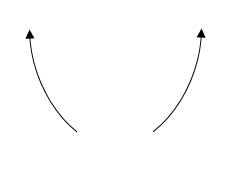
\includegraphics[width = 0.3\textwidth]{../Figures/polyEndBehaviorCopyCA.png}\item 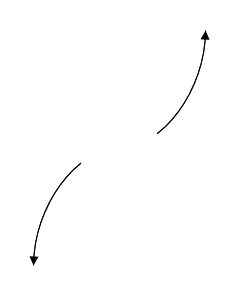
\includegraphics[width = 0.3\textwidth]{../Figures/polyEndBehaviorCopyDA.png}\end{multicols}\item None of the above.
\end{enumerate} }
\litem{
Construct the lowest-degree polynomial given the zeros below. Then, choose the intervals that contain the coefficients of the polynomial in the form $x^3+bx^2+cx+d$.\[ -4 + 2 i \text{ and } -3 \]\begin{enumerate}[label=\Alph*.]
\item \( b \in [-17, -4], c \in [38, 48], \text{ and } d \in [-61, -58] \)
\item \( b \in [-4, 7], c \in [6, 11], \text{ and } d \in [7, 18] \)
\item \( b \in [6, 12], c \in [38, 48], \text{ and } d \in [59, 70] \)
\item \( b \in [-4, 7], c \in [-3, 2], \text{ and } d \in [-8, -3] \)
\item \( \text{None of the above.} \)

\end{enumerate} }
\litem{
Describe the end behavior of the polynomial below.\[ f(x) = -2(x - 2)^{2}(x + 2)^{7}(x + 8)^{3}(x - 8)^{5} \]\begin{enumerate}[label=\Alph*.]
\begin{multicols}{2}\item 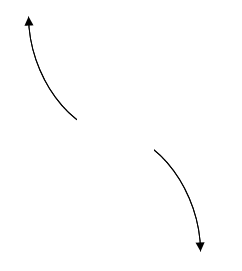
\includegraphics[width = 0.3\textwidth]{../Figures/polyEndBehaviorAA.png}\item 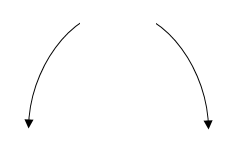
\includegraphics[width = 0.3\textwidth]{../Figures/polyEndBehaviorBA.png}\item 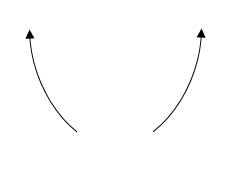
\includegraphics[width = 0.3\textwidth]{../Figures/polyEndBehaviorCA.png}\item 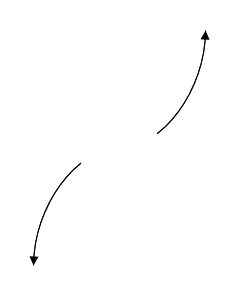
\includegraphics[width = 0.3\textwidth]{../Figures/polyEndBehaviorDA.png}\end{multicols}\item None of the above.
\end{enumerate} }
\litem{
Construct the lowest-degree polynomial given the zeros below. Then, choose the intervals that contain the coefficients of the polynomial in the form $x^3+bx^2+cx+d$.\[ -2 - 4 i \text{ and } -2 \]\begin{enumerate}[label=\Alph*.]
\item \( b \in [-11, -3], c \in [27.08, 28.99], \text{ and } d \in [-40.7, -36.4] \)
\item \( b \in [-3, 5], c \in [4.37, 7.77], \text{ and } d \in [5.9, 8.6] \)
\item \( b \in [2, 15], c \in [27.08, 28.99], \text{ and } d \in [36.9, 41.9] \)
\item \( b \in [-3, 5], c \in [2.08, 5.16], \text{ and } d \in [2.9, 4.7] \)
\item \( \text{None of the above.} \)

\end{enumerate} }
\litem{
Construct the lowest-degree polynomial given the zeros below. Then, choose the intervals that contain the coefficients of the polynomial in the form $ax^3+bx^2+cx+d$.\[ 5, \frac{-7}{4}, \text{ and } \frac{-4}{5} \]\begin{enumerate}[label=\Alph*.]
\item \( a \in [19, 30], b \in [-50, -45], c \in [-227, -224], \text{ and } d \in [140, 146] \)
\item \( a \in [19, 30], b \in [46, 52], c \in [-227, -224], \text{ and } d \in [140, 146] \)
\item \( a \in [19, 30], b \in [142, 154], c \in [277, 289], \text{ and } d \in [140, 146] \)
\item \( a \in [19, 30], b \in [77, 83], c \in [-125, -118], \text{ and } d \in [-140, -135] \)
\item \( a \in [19, 30], b \in [-50, -45], c \in [-227, -224], \text{ and } d \in [-140, -135] \)

\end{enumerate} }
\end{enumerate}

\end{document}